\documentclass[10pt, mathserif]{beamer} % font and normalsize
\usetheme{Antibes}
\usepackage{xeCJK}
%\usepackage{charter}
\usepackage{comment}
%\usepackage[colorlinks=false]{hyperref}

\usepackage[title,titletoc]{appendix}
\usepackage{pagecolor}
\usepackage{amsmath}
\usepackage{amsfonts}
%\usepackage{ulem}
%\usepackage{siunitx}
%\sisetup{per=slash, load=abbr}

%\mode<presentation>
%{
%    \setbeamercovered{dynamic}  % translucent when using pause
%    \setbeamertemplate{navigation symbols}{}    % hide navigation bars
%    \setbeamertemplate{caption}[numbered]   % numerate captions
%    \setbeamertemplate{background}{\includegraphics[height=\paperheight]{ISEE.pdf}} % set background image
%    \setbeamertemplate{footline}{\footnotesize \insertframenumber/\inserttotalframenumber \hfill}   % display page number at bottom left corner
%}



\usepackage{pgfplots}
\usetikzlibrary{positioning}
\usetikzlibrary{fit}
\usetikzlibrary{snakes}
\usetikzlibrary{shapes.geometric}
\usetikzlibrary{patterns}
\usetikzlibrary{shapes,arrows,chains}
\usepgfplotslibrary{patchplots,colormaps}
\usetikzlibrary{calc}
\usetikzlibrary{positioning, fit}
\usetikzlibrary{backgrounds}
\usetikzlibrary{intersections}


%\setCJKmainfont[BoldFont = STSongti-SC-Bold]{STSongti-SC-Regular}

\newcommand{\reffig}[1]{图\ref{#1}}
\newcommand{\refsec}[1]{\S \ref{#1}}


\newcommand{\nrcore}{Core Nebulas Rank}
\newcommand{\nrext}{Extended Nebulas Ranks}
\newcommand{\dom}{{\; \texttt{dom}\;}}
\renewcommand{\figurename}{图}

%\setCJKsansfont[BoldFont = STHeitiSC-Medium]{STHeitiSC-Light}



\usepackage{charter}
\usepackage{fullpage}
\usepackage[colorlinks=false]{hyperref}
\usepackage{ifthen}
\usepackage{comment}
\usepackage[title,titletoc]{appendix}
\usepackage{pagecolor}
\usepackage{amsmath}
\usepackage{amsfonts}
%\usepackage[normalem]{ulem}
\usepackage{siunitx}
\usepackage{amsthm}
\sisetup{per=slash, load=abbr}

\usepackage{pgfplots}
\usetikzlibrary{positioning}
\usetikzlibrary{fit}
\usetikzlibrary{snakes}
\usetikzlibrary{shapes.geometric}
\usetikzlibrary{patterns}
\usetikzlibrary{shapes,arrows,chains}
\usepgfplotslibrary{patchplots,colormaps}
\usetikzlibrary{calc}
\usetikzlibrary{positioning, fit}
\usetikzlibrary{backgrounds}
\usetikzlibrary{intersections}

\newcommand{\whitepaper}[1]{\begin{center}\fbox{\parbox{0.75\textwidth}{{\small
#1}}}\end{center}}

\newcommand{\pcolor}{yellow!25}

\usepackage{setspace}
\usepackage{algorithm2e}
\bibliographystyle{ieeetr}

\usepackage{geometry}
\geometry{left=3cm,right=3cm,top=1.6cm,bottom=3cm,headheight=0pt,headsep=1.5em}
\usepackage{fancyhdr}
\pagestyle{fancy}
\chead{
\includegraphics[scale=0.2]{../common/Nebulas.png}}  %在此处插入logo.pdf图片 图片靠左
\lhead{} % 页眉中间位置内容
\rhead{}
%\setlength{\topskip}{1em}



\begin{document}

\title[abbreviation]{ 星云指数}
\author{ Nebulas Research Team}

\date{June, 2018}

\AtBeginSection[]
{
\begin{frame}
    \tableofcontents[currentsection, currentsubsection]
\end{frame}
}

\begin{frame}
    \titlepage	% make the cover page here
\end{frame}

% !TEX root = main.tex

\section{Introduction}

As blockchain technologies continue to evolve, more and more industries benefit from \emph{decentralization}, which
is the core of blockchain systems. For example, Bitcoin, the origin of
blockchain, has proven its significance to digital assets, while Ethereum has
proven how important is decentralization to DApps. As time progresses there are more and more
blockchain projects exploring how they can leverage decentralization.

Obviously, the backbone of decentralization in blockchain is both its openness and inherent features of anonymity.


Yet, openness and anonymity obstruct the emergence of value
measurements~\cite{meiklejohn2013fistful}. There are two aspects of this obstruction. First, it is
difficult to infer whether multiple accounts belong to the same user, rendering it difficult to build a mechanism like HTTP Cookies~\cite{Cookie}, or to use
traditional data analysis technologies to understand user characteristics.
Second, the openness of blockchain makes it vulnerable to manipulation,
especially for value measurements. Attackers can easily attain details about the
value measurements, and figure out weakness of the whole system. This
largely differs from traditional value measurements which are either closed or
independent.

We believe that the effective value measurement is the foundations of
blockchain's prosperity. Both the lack of and ineffectiveness of value measurement may confine blockchains to a limited set of use cases.

First of all, we need a methodology to quantify the value of data,
applications and accounts on blockchains. The root cause is cooperations on
blockchain keeps scaling up, and the requirements of efficiency
keeps growing. Without value measurement, such collaboration may be negatively affected.

Second, blockchain technology remains at a very early stage of development and use-case, and the value of data
and assets on the blockchains is still underground and waiting to be found.
Effective value measurements will uncover the value and empower more applications and enable more application scenarios, for example, loans, credit, data search, personalized recommendation and cross-chain interaction.

Third, incentives, which is based on value means, are necessary to sustaining a healthy blockchain ecosystem. Without effective value measurements, incentives may lead a blockchain system to corruption and eventual collapse.

As a conclusion, an effective value measurement for blockchain needs to be:
\begin{itemize}
\item{\textbf{Truthful.}} The rank needs to measure some characteristic of a blockchain system, and thus can be trusted in some way;
\item{\textbf{Fair.}} This means the rank need to be manipulation-resistant, and it is the core of the rank algorithm;
\item{\textbf{Diverse.}} There will be different ranking requirements from different applications on blockchain, thus a quality ranking algorithm should cover different scenarios.
\end{itemize}

We believe Nebulas Rank shall be an effective value measurement for
blockchains.

For truthfulness, we define Nebulas Rank to be the quantification of an account's
contribution to the blockchain system after considering many different
metrics.

We believe that cryptocurrencies should have the attributes of money, in particular,
three functions of money: medium of exchange, store of value, and unit of
account. Blockchains themselves are economic systems and the classical monetary theory still has the instruction value. Furthermore, we believe the value of cryptocurrencies comes from the liquidity. Specifically, each transaction between users increases the liquidity of cryptocurrencies, and endows the value of cryptocurrency eventually. Thus, the on-chain transactions are effective and natural data sources for effective value measurement.


To evaluate the effectiveness of Nebulas Rank, we calculate the sum of all
accounts' Nebulas Rank on Ethereum, and compare it with the market capitalization
given by \texttt{coinmarketcap.com}. Our evaluation shows strong
correlation between them, approximately $0.84$. That means Nebulas is effective at measuring
accounts' contribution at the micro-level, while also being able to measure the
value of blockchain systems at the macro-level.

For fairness, we involve a special function to resist manipulation, and our analysis demonstrates its performance to be manipulation-resistant.

Based on the theory of Nebulas Rank, we can further divide Nebulas Rank into Core Nebulas
Rank and Extended Nebulas Rank for different applications and scenarios.

Core Nebulas Rank defines the algorithm to calculate an account's contribution
to the whole blockchain system over a certain period of time. And such
calculate involves two factors: the median stake of an account over a certain
period, and the in-and-out degree of the account over a certain period.

Extended Nebulas Rank is suited to different applications and scenarios,
and it is closely based on Core Nebulas Rank. For example, we show how to rank smart
contracts based on Core Nebulas Rank; we also show how to extend Core Nebulas Rank to a multi-dimensional vector.


Besides theory and methodology of Nebulas Rank, we also present our
consideration on how to implement Nebulas Rank, including whether to
place ranking scores on-chain, how to update the algorithm of Nebulas Rank,
and our future planned work on Nebulas Rank.

\whitepaper{
  Special Hint:
  The content in this yellow paper may be different from the description in our
  whitepaper (version 1.02 released on April 2018)~\cite{Nabulas}. This is because we keep
  thinking and verifying the algorithm in our whitepaper. And now we are more
  confident and capable to make it more rigorous. We use a different format
  (like this paragraph) to emphasize the relevant updates presented in this yellow paper.

}

% !TEX root = main.tex

\section{背景及相关技术}
%\subsection{讨论}
%主要参考nem白皮书,背景:缺少价值尺度
%pos:stake
%pow:computation power
%poa:
%poi:

%neb:用statke,鼓励资产流通,需要引入流通性,but 容易受到sybil attack
%现有算法 e.g. page rank

%我们的工作基于前人的工作

本章主要介绍区块链发展背景以及相关技术。鉴于目前的区块链生态之上价值衡量尺度的缺失,我们进一步讨论了经典排名算法在区块链领域应用的情况以及其缺陷。

\subsection{区块链发展情况}
2008年10月,中本聪(Satoshi Nakamoto)公开发表比特币白皮书~\cite{Nakamoto2008}。比特币作为区块链的太初应用,践行了其作为“一个去中心化电子现金系统”的初衷。 比特币的产生不依赖于任何机构,而是根据特定算法,依靠大量计算产生,保证了比特币网络分布式记账系统的一致性。

通过特定的脚本语言,我们可以利用比特币实现第三方支付交易、高效小额支付(efficient micro-payments)等功能。同时,除去基本的货币属性,出现了许多以比特币为参照的试验品。例如早期的域名币(Namecoin)~\cite{Namecoin}提供了一种去中心化的域名系统DNS以及基于“货币染色(Colored coins)”的开放资产项目(OpenAssets)~\cite{OpenAssets},其本质都是模仿比特币的可追溯性,复制一份智能资产。

%后续其他数字货币支持赌博、股票发行、市场预测等。

很遗憾的是,比特币脚本语言的设计存在很多缺陷,如仅支持较少指令,且并不具备图灵完备性,这使得其应用场景受限。随着区块链技术研究的不断深入,涌现了更多后继者,尝试拓展和添加更多与应用程序相关的功能。其中最令人瞩目的实现是以太坊(Ethereum)~\cite{buterin2013ethereum},以太坊突破性地提供了图灵完备的智能合约(Smart Contracts),从而大幅拓展了应用场景。

智能合约是区块链系统中可以用技术手段来强制执行的合约,以太坊智能合约运行在以太坊虚拟机(Ethereum Virtual Machine)上,以太坊虚拟机不受任何实体控制,通过共识算法来验证合约本身及其输出的完整性。

基于以太坊智能合约,人们得以开发能实现复杂功能的分布式应用(DApp)。除了基本交易功能外,DApp为众多领域提供了解决方案,如投票、众筹、借贷、知识产权等。

以太坊成功拓展了区块链的可能性,但以太坊缺少价值衡量标准,在应用落地时遇到了阻碍,至今没有杀手级应用诞生。

对于支持智能合约的区块链系统,其账户通常包括外部账户(Externally owned account,EOA)和智能合约账户,对于这两类账户目前尚缺少合理的评价指标。同时,在诸多交易以及智能合约的调用过程中,隐藏着难以估计的信息。后者相比传统交易数据,往往具有更多维度,因此也无法使用传统价值衡量标准评估。

其实,早在2015年,Chris Skinner便提出了“价值网络(value web)”的理念~\cite{ChrisSkinner},其中提到一个价值经济系统(Value ecosystem)应包括价值交换(value exchanges)、价值存储(value stores)以及价值管理系统(value management systems)三部分,缺一不可。同时Chris也指出,对于比特币等数字加密货币来说,价值网络的衡量相比传统社会价值有着明显不同,挑战更大。




%现在链超多,跨链需要衡量价值。。。


\subsection{图中节点的排名算法}
由于智能合约的引入,当前以以太坊为代表的新一代区块链项目不仅仅是电子货币交易平台,而是在此之上建立了复杂庞大的经济体系。尚不存在一个合理的方式去评估链上实体(例如用户地址)的价值。例如,目前我们无法知晓哪些实体为整个区块链生态贡献较大?又应如何衡量这类贡献?

在此,需要先提到一个在传统互联网领域大家都比较熟悉的价值衡量标准:PageRank算法~\cite{page1999pagerank}。作为Google早期的核心算法,PageRank设计初衷是用于解决链接分析中网页排名问题。随着国内外学者的深入研究,PageRank算法被广泛应用于其它方面,例如学术论文的重要性排名、网络爬虫、关键词与句子的抽取,以及基于PageRank的社交用户影响力排名研究等等。

学术界也已有将PageRank算法应用于区块链的研究,比如Fleder、Kester、Pillai等人~\cite{Fleder2015} 使用 PageRank 来帮助发现感兴趣的比特币地址,并分析这些地址的活 动。但他们的工作仍然将人工主观分析作为主要方法,PageRank 只起到辅助作用。

作为诞生于互联网2.0时期的经典排名算法,PageRank算法应用于在线社会网络影响力评估存在局限性。此后涌现出了一些其它在PageRank算法基础上进行改良的研究,其中较为著名的包括LeaderRank算法 ~\cite{Li2014},它是 PageRank 的一种拓展形式。在 PageRank 中,每个节点都有相同的随机跳转概率,而LeaderRank 是对跳转概率简单有效的改进。通过在网络中添加 背景节点和加权的双向链接,可以使得不同节点具有不同的随机跳入和跳出概率。

LeaderRank算法的基本思想是在整个网络已有节点外另外增加一个背景节点(Ground Node),并且将其与已有所有节点建立双向连接,使得N+1个节点的新网络成为一个强连通网络,在此基础上基于类似PageRank算法计算可以得到原有N个节点的“重要性”排序。
而LeaderRank也存在一定局限性,其只考虑了节点之间的关系(即网络结构),通过迭代得出最后影响力排名,缺乏对用户行为的衡量。

需要指出的是,PageRank类排名算法无法应对女巫攻击(sybil attacks)~\cite{cheng2006manipulability},后者是指攻击者通过创建大量的假名标识来破坏对等网络的评价系统,从而获得虚假的高重要性评分。


和 Nebulas Rank 最相关的项目是 NEM~\cite{nem},不同于比特币的Proof-of-Work以及以太坊的 Proof-of-Stake共识策略,NEM设计了 Proof-of-Importance 共识机制,其中排名算法 NCDawareRank ~\cite{Nikolakopoulos2013}利用了网络拓扑的社群效应。Proof-of-Importance 使用 SCAN ~\cite{xu2007scan}\cite{shiokawa2015scan}\cite{chang2017mathsf}作为社群聚类算法。虽然社区结构在交易网络的确存在并且可以帮助应对欺诈节点,却 无法保证同一个实体对应节点一定可以映射到相同社群,因此利用社区划分的结果会提供一定的可操纵空间。

%Nebulas Rank 的加权机 制部分参考了 Li et al. [32] 的设计,使得入度更大的点更有可能被随机跳转到达。通过添加 LeaderRank 算法中的背景节点,可以取得更符合区块链场景的排名结果。

\subsection{对抗操纵}
提升可信性,即具备抵抗操纵的能力,是核心星云指数最重要同时也是最具挑战的目标。

Hopcroft等人发现,在存在恶意操控的情况下,PageRank无法有效衡量用户的影响力~\cite{hopcroft2007manipulation}。Zhang等人指出,在社交网络中,即便建立了节点的影响评价指标,攻击者仍然能够有效削弱其他非僵尸用户的影响力~\cite{zhang2016truetop}。
比如针对PageRank算法的典型女巫攻击:环形攻击(two-loop attack)就是一例。以女巫节点$s$发起到目的节点
$v_j$以及从$v_j$返回到$s$的Random walk(尽可能多地访问其它节点),从而增加$v_j$的访问概率。

这是因为从本质上而言,PageRank类算法依赖于网络拓扑结构对用户进行排名,而在对称网络(symmetric Network)下,恶意操纵者非常容易通过构建镜像网络来获取同样甚至更高的影响力~\cite{cheng2005sybilproof}~\cite{cheng2006manipulability}。


在区块链生态中,部分恶意操纵的手段通常有以下几种:
\begin{enumerate}
\item 环形转账,攻击者沿环形拓扑,让同一笔资金不断流过对应的边,以提高边权;
\item 向其它任意账户转钱,提高出度,并且提高资金流出的传播性;
\item 控制多个账户形成独立分支,伪造中心节点;
\item 频繁同权威交易所账户交易,多次在交易所账户中取入取出同一笔资金,获得较好的网络结构位置。
\end{enumerate}

因此我们在设计核心星云指数时,需要考虑到上述情况,来保证核心星云指数的公平性。




%博弈论相关工作了解一下
%看着还行,但是假设太强,抗操纵性不行的。


\section{区块链经济模型}
\begin{frame}
	\frametitle{加密数字货币表示}
  加密数字货币系统,表示为$(\mathcal{L}, \mathcal{U})$,其中
  \begin{align}
  \mathcal{L} = (\mathcal{A}, \mathcal{D}, \mathcal{T})
  \end{align}
  \begin{align}
  \mathcal{D} = \{a \rightarrow d, a{\in}\mathcal{A}, d{\in}R^*\}
  \end{align}
  \begin{align}
  \mathcal{T} = \{(s, t, w, \tau)\}
  \end{align}
一个账户与用户只能被唯一的用户控制,一个用户能够控制多个账户
\begin{align}
u \dom a. \quad u\in \mathcal{U}, a\in \mathcal{A}
\end{align}
\begin{align}
A(u) = \{\forall a\in \mathcal{A} : u \dom a\}
\end{align}
\begin{align}
\forall u_1, u_2 \in \mathcal{U} : A(u_1) \cap A(u_2) = \phi
\end{align}
\end{frame}

\begin{frame}
\frametitle{加密数字货币模型}
数字货币应该具备货币属性,即交换媒介、计价单位和价值储藏手段。
经典货币数量论:
\begin{align}
M\times V=P\times Y
\label{eq:currency}
\end{align}
而在加密数字货币中,可以写为:
\begin{align}
(M + \Delta{m}) \times \frac{\sum_{(s, t, w, \tau)\in \mathcal{T}}{w}}{M} = P \times Y
\label{eq:cur_ext}
\end{align}
更进一步的
\begin{align}
Y=\sum_{a\in \mathcal{A}} \mathcal{C}(a)
\end{align}
\noindent 其中$\mathcal{C}(a)$表示账户$a$对整个经济产量的贡献,即星云指数。
\end{frame}

\begin{frame}
\frametitle{星云指数}
星云指数衡量了一个账户对经济系统的贡献。数字货币的发展依赖于社区的发展,因
此,我们认为量化社区中每个账户对于经济总量的贡献,为正确的激励提供了必要的基
础。
\begin{itemize}[<+->]
\item 核心星云指数
\item 扩展星云指数
\end{itemize}
\end{frame}

% !TEX root = main.tex
\section{核心星云指数}

核心星云指数用于衡量{\textbf{一段时间内}}用户对整个经济体的贡献。
精确地计算这一指标是十分困难的,因此,我们使用了近似算法。
在该近似算法中,我们考虑了两个重要的因素,即账户持有的币龄和账户在交易网络中的位置信息。在稍后的评测中,我们将证明这种近似算法的有效性。


我们使用一段时间内链上的交易记录作为核心星云指数的数据来源。
对于一段时间$[t_0\ −\ T,\ t_0]$内的交易记录,可以描述为集合
\begin{align}
\Theta(t_0) = \{(s, t, w, \tau)\ |\ t_0 - T \le \tau \le t_0\ \land \ w > 0 \land s \neq t \}
\end{align}
\noindent 基于$\Theta(t_0)$,我们可以构造有向加权图,其中节点为账户地址,从节点$s$到节点$d$的有向边是一次交易,
边的权值为$w$,边的时间为$\tau$。


对于账户$a \in \mathcal{A}$,其核心星云指数$\mathcal{C}(a)$的计算基于$\Theta(t_0)$,即
\begin{align}
\mathcal{C}(a) = \Omega(\beta(a)) \times{} \Psi(\gamma(a))
\label{eq:rank}
\end{align}
\noindent 其中$\beta(a)$为一段时间内账户$a$持有资产的中值;$\gamma(a)$为账户$a$在一段时间内的出入度指标。

%{我们分别考虑式~\ref{eq:rank}中的三个问题,资产中值$\beta(a)$的计算,出入度指标$\gamma(a)$的计算,以及计算函数$\Omega$及$\Psi$的选择。}

%{\color{gray}注意,我们并未使用技术白皮书中的计算方法。说说原因,}

\whitepaper{相比星云技术白皮书~\cite{Nabulas}中对于星云指数的计算方法,我们做了如下改动:\\
1.在构造交易图时取消了采取最高$K$个交易额作为权值;\\
2.取消了LeaderRank中通过计算背景节点有向边权重来获取重要性评分的方式。\\
首先,我们在计算出入度指标$\beta$时采用了去环处理,因此已经可以抵抗环形转账攻击,并同时保留边的强度信息。对于存在同构图的拓扑结构,PageRank等对称函数(包括LeaderRank)被证明无法有效抵抗女巫攻击~\cite{cheng2005sybilproof}。因此在本黄皮书中我们没有采用类拓扑排名策略。在~\refsec{sec:function}中我们构造的非对称计算函数~\ref{eq:rank-param}将可以有效降低伪造低收入节点的收益。}

下面,我们将分别考虑~\ref{eq:rank}中的三个问题:资产中值$\beta(a)$的计算、出入度指标$\gamma(a)$的计算,以及函数$\Omega$及$\Psi$的选择。

\subsection{资产中值$\beta(a)$}
对于时间段$[t_0\ −\ T,\ t_0]$,区块链系统中存在$n$个区块,记为
\[
B_0, B_1, \dots, B_n
\]
\noindent 其中$B_{i}$ 为$B_{i+1}$的父块。对于账户$a \in \mathcal{A}$,其在每个区块结束后,
其相应的账户余额为
\[
d^a_0, d^a_1, \dots, d^a_n
\]
上述序列按从小到大排序后可以得到
\[
d^a_{(0)}, d^a_{(1)}, \dots, d^a_{(n)}
\]
其中$d^a_{(i)} < d^a_{(i+1)}, 0\le i \le {n-1}$,由此,可以得到
\begin{align}
\beta(a) = \left\{ \begin{array}{rcl}
{d^a_{(k)}} & \mbox{for} & n=2\times{}k, k=1, 2, 3, \ldots \\
{(d^a_{(k)} + d^a_{(k+1)})/2} & \mbox{for} & n=2\times{}k + 1, k=1, 2, 3, \ldots
\end{array}\right.
\end{align}
资产中值一定程度上代表了“币龄”,即账户中需要至少持有该资产一半以上的时间。

\subsection{出入度指标$\gamma(a)$}
考虑到恶意操控者会利用“环形转账”行为提升自己的出入度指标,因为对于出入度指标的计算首先需要对交易图进行“去交易环”处理。交易环(forwarding loop)是指一组按时间顺序进行的交易行程的环路。
一个交易环在节点$v$开始并结束,是交易图中边的集合,记为$H(v)$,即,
\[
H(v) = \{(v, v_1, w_1, \tau_1), (v_1, v_2, w_2, \tau_2), \dots, (v_i, v_{i+1}, w_{i}, \tau_i), \dots, (v_n, v, w_{n+1}, \tau_{n+1})\}
\]
\noindent 其中,$\forall 1\le i \le n : \tau_i \le \tau_{i+1} $。
\noindent 如~\ref{fig:loop}所示,包含了一个交易环,注意,其中$(v_1, v_2, 100, 5)$并不包含在交易环中。

\begin{figure}
\centering
  \begin{tikzpicture}
\pgfmathsetmacro{\XTD}{3.8}
\pgfmathsetmacro{\XMD}{1.2}
\pgfmathsetmacro{\YTD}{3.8}


\tikzset{
  node/.style={draw, circle, on grid, align=center, minimum height=2ex},
  thread/.style={draw, rectangle, on grid, align=center,color=gray!30,
  fill=gray!30,
  rounded corners,
  minimum height=3ex,fit=#1},
}

\node[node] (v) at (0, 0) {$v$};
\node[node] (v1) at (0, \YTD) {$v_1$};
\node[node] (v2) at (\XTD, \YTD) {$v_2$};
\node[node] (v3) at (\XTD, 0) {$v_3$};

\draw[->,>=stealth'] (v) to [out=135, in=225] node[left, midway] {$w=100$,$\tau=1$} (v1);
\draw[->,>=stealth'] (v1) to [out=45, in=135] node[above, midway] {$w=10$,$\tau=2$} (v2);
\draw[->,>=stealth'] (v1) to [out=315, in=225] node[below, midway] {$w=100$,$\tau=5$} (v2);
\draw[->,>=stealth'] (v2) to [out=315, in=45] node[right, midway] {$w=10$,$\tau=3$} (v3);
\draw[->,>=stealth'] (v3) to [out=225, in=315] node[below, midway] {$w=10$,$\tau=4$} (v);

\node at (2.5*\XTD, 0.5*\YTD) {
$\begin{aligned}
     H(v) = \{&(v, v1, 100, 1),\\
     &(v1, v2, 10, 2), \\
     &(v2, v3, 10, 3), \\
     &(v3, v, 10, 4) \}
  \end{aligned}$};
\end{tikzpicture}

\caption{loop\label{fig:loop}}
\end{figure}

\begin{figure}
\centering
\begin{tikzpicture}
\pgfmathsetmacro{\XTD}{3.8}
\pgfmathsetmacro{\XMD}{1.2}
\pgfmathsetmacro{\YTD}{3.8}


\tikzset{
  node/.style={draw, circle, on grid, align=center, minimum height=2ex},
  thread/.style={draw, rectangle, on grid, align=center,color=gray!30,
  fill=gray!30,
  rounded corners,
  minimum height=3ex,fit=#1},
}

\node[node] (v) at (0, 0) {$v$};
\node[node] (v1) at (0, \YTD) {$v_1$};
\node[node] (v2) at (\XTD, \YTD) {$v_2$};
\node[node] (v3) at (\XTD, 0) {$v_3$};
\draw[->,>=stealth'] (v) to [out=135, in=225] node[left, midway] {$w=90$,$\tau=1$} (v1);
\draw[->,>=stealth'] (v1) to [out=315, in=225] node[below, midway] {$w=100$,$\tau=5$} (v2);

\end{tikzpicture}
\caption{\reffig{fig:loop}去掉交易环后的交易图 \label{fig:no-loop}}
\end{figure}


在找到交易环后,需要进行去交易环处理。假设系统中存在$n$个交易环,按照交易环在交易图中出现的顺序记为
\[
H^1(v_1), H^2(v_2), \dots, H^n(v_n)\]
\noindent 其中,$H^i(v_i)$中交易金额最小的交易为 $(s^i_m, t^i_m, w^i_m, \tau^i_m)$,即
\[
\forall (s^i, t^i, w^i, \tau^i) \in \mathcal{T} : w^i \ge w^i_m
\]
\noindent 然后,需要依次将$H^i(v_i)$中所有的交易减去相应的最小交易量$w^i_m$,
如果新的交易量为0,则移除该交易,即
\[
\mathcal{E}((s, t, w, \tau), w_m) = \left\{ \begin{array}{rcl}
(s, t, w-w_m, \tau) & \mbox{if} & w \ne w_m \\
\phi & \mbox{if} & w = w_m
\end{array}\right.
\]
\begin{align}
\Theta^{\prime}(t_0)=\Theta(t_0)-H^i(v) \cup \{\mathcal{E}(t), t\in H^i(v_i)\} \quad i = 1, 2,\dots, n
\end{align}
\noindent 如~\reffig{fig:no-loop}所示,为~\reffig{fig:loop}去掉交易环之后的交易图。


%在去除所有的交易环后,对交易图中的每个节点,我们仅保留交易量最高的$k$个出边及入边,由此得到新的交易图$\Theta^{\prime\prime}(t_0)$。

记节点$v$的转入金额为$p(v)$,则
\begin{align}
p(v) = \sum_{(s_i, v, w_i, \tau_i) \in \Theta^{\prime}(t_0)}{w_i}
\end{align}
\noindent 同理,节点$v$的转出金额有
\begin{align}
q(v) = \sum_{(v, t_i, w_i, \tau_i) \in \Theta^{\prime}(t_0)}{w_i}
\end{align}
\noindent 由此,
对于节点$v$,其出入度指标$\gamma(v)$为

\begin{align}
\mathcal{G}(v) = (p(v) + q(v)) \cdot e^{-2\sin^2{(\frac{\pi}{4} - \arctan\frac{q(v)}{p(v)})}}
\end{align}
\noindent 该函数图形如~\reffig{fig-surf}所示。
\begin{figure}
  \centering
  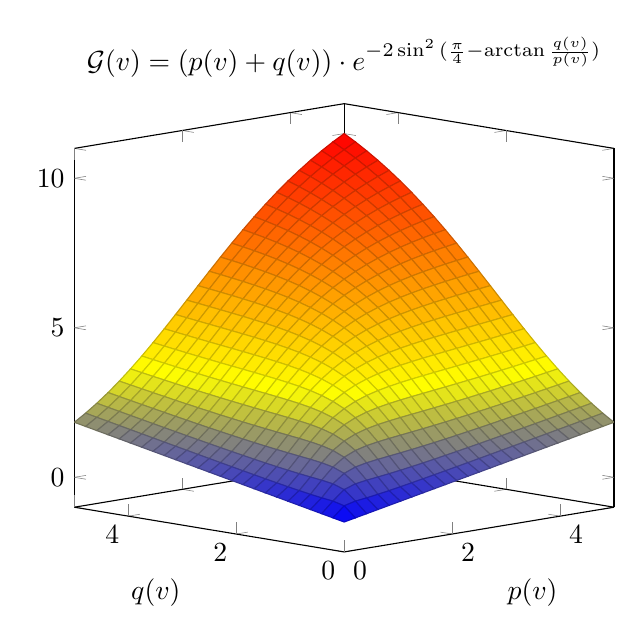
\begin{tikzpicture}[
    declare function={tf(\x)=(pi/4-rad(atan(\x)));},
    declare function={func(\x,\y)=sin(tf(\y/\x)*180/pi);}
]
\begin{axis}[
    view={315}{10},
    title={$
\mathcal{G}(v) = (p(v) + q(v)) \cdot e^{-2\sin^2{(\frac{\pi}{4} -
\arctan\frac{q(v)}{p(v)})}}$},
    xlabel=$p(v)$,
    ylabel=$q(v)$,
]

\addplot3 [
        surf,
        domain=0:5,
        domain y=0:5,
    ] {(x+y)*exp((-2)*(func(x,y))^2)};
\end{axis}
\end{tikzpicture}

\caption{出入度计算函数曲线 \label{fig-surf}}
\end{figure}

\begin{align}
\gamma(v) = (\frac{\theta\cdot \mathcal{G}(v)}{\mathcal{G}(v) + \mu})^{\lambda}
\end{align}
\noindent 其中$\theta, \mu, \lambda$为待定的参数。


\subsection{Wilbur函数 \label{sec:function}}
考虑到不同的使用场景及不同的性质,星云指数的计算是十分复杂的,然而,我们可以总结出一般意义上的星云指数计算函数的特征。

在此我们将星云指数的计算函数命名为Wilbur Function\footnote{女巫攻击(Sybil Attack)命名的来源于上世纪七十年代的美国系列电影《Sybil》,剧中患有人格分裂症的小女孩名叫Sybil,而治疗她的心理医生则名叫Dr. Cornelia Wilbur。},记为\(f(x)\),其中\(x\)
为星云指数需要参考的因素,可以为持有的余额、币龄或账户的出入度。$f(x)$需要满足两个性质:

\begin{property}
\label{prop:one}
对于任意大于$0$的两个输入变量$a$,$b$,其计算函数之和小于其和的计算函数。
%对于任意输入$x$,将其拆分后的计算函数之和小于原计算函数。
\end{property}

\begin{align}
f(a+b)>f(a)+f(b) \quad a>0,b>0
\end{align}

\begin{property}
\label{prop:two}
当任意大于$0$的两个输入变量趋近于无穷大时,其计算函数之和趋近于其和的计算函数。
\end{property}

\begin{align}
\lim\limits_{a \to \infty, b\to \infty} f(a+b) = f(a) + f(b)\quad a>0, b>0
\end{align}

\noindent 上述特性保证了在给定交易行为的情况下,用户通过控制多个账户实现该交易行为的收益小于通过单一账户实现交易的收益,同时当用户资产足够大时,其拆分账户交易的损失可以忽略不计。

\noindent 满足上述两个性质的函数有很多,在此,我们仅给出一个满足上述性质的函数,该函数的图形如~\reffig{fig-nr}所示。
\begin{align}
f(x) = x/(1 + e^{a + b\cdot x}) \quad a>1,b<0
\end{align}
\noindent {证明:详细见附录~\ref{sec:appendix_proof}}

\begin{figure}
\centering
\begin{tikzpicture}[
    declare function={func(\x,\mu) = (\x / (1 + exp(\mu-\x)));},
    declare function={linefunc(\x) = \x;}
]
\begin{axis}[
    axis lines=left,
    enlargelimits=upper,
ticks=none,axis x line=bottom,axis y line=left,xlabel={Nebulas Rank Factor},
  ylabel={星云指数},
      legend pos=north west,
legend style={fill=none}
]
\addplot [dashed, domain=0:10, blue] {linefunc(x)};
\addplot [smooth, domain=0:10, red] {func(x,3)};
\addlegendentry{$f(x)=x$}
\addlegendentry{$f(x)=x/(1 + e^{a + b\cdot x})$}
\end{axis}
\end{tikzpicture}
\caption{星云指数计算函数曲线 \label{fig-nr}}
\end{figure}


\vspace{2em}
综上,式~\ref{eq:rank}可以进一步写为

\begin{align}
\label{eq:rank-param}
\mathcal{C}(v) =  \frac{\beta(v)}{1+e^{a + b \cdot \beta(v)}} \cdot \frac{\gamma(v)}{1+e^{c + d \cdot \gamma(v)}}
\end{align}
\noindent 其中,$a, b, c, d$为待定的参数。

为了验证该函数的有效性,我们根据以太坊中的数据,计算了以太坊中地址的星云指数,并根据其市值变化计算了两者的相关性。测试数据包括了以太坊从2017年5月1日起至2017年6月30日(3629091区块至3955158区块)的所有交易记录,以及ETH日均价格(对美元)和日均总交易量~\cite{coinmarketcap}。


~\reffig{fig-eth-simu}表示了以太坊的市值与星云指数随时间变化趋势,如图所示,其中黑色标记实线为通过ETH日均交易量以及ETH日均价格计算得出的以太坊市值(对美元),而红色实线则是根据公式~\ref{eq:rank-param}计算所有以太坊用户的星云指数之和。

可以看出,星云指数能够有效反映以太坊市值变化,二者的相关系数(Correlation coefficient)为0.84427,$p$值(p-value)为$4.48\times{}10^{-17}<0.001$。说明函数~\ref{eq:rank}能够有效表示用户对整个经济体的贡献,即体现出星云指数的真实性。


\begin{figure}
\centering
\begin{tikzpicture}
  \begin{axis}[
  axis y line*=left,
  axis x line=none,
%ticks=none,
ylabel={以太坊市值(美元)},
%xtick={0,10,20,30,40,50,60},
%xlabel={时间(天)}
legend style={fill=none}
    ]
\addplot[smooth, mark=., color=red] table [x=day, y=nr, col sep=comma]
    {../common/eth_simu.csv};
\label{plot_one}

\end{axis}
  \begin{axis}[
%ticks=none,
legend pos=north west,
%ylabel={星云指数},
xlabel={时间(天)},
xtick={0,10,20,30,40,50,60},
ytick={1,2},
axis y line*=right,
legend style={fill=none}
    ]
    \addlegendimage{/pgfplots/refstyle=plot_one}\addlegendentry{星云指数}

    \addplot[smooth, mark=x] table [x=day, y=cap, col sep=comma]
    {../common/eth_simu.csv};
    \label{plot_two}
      \addlegendentry{以太坊市值}
\end{axis}

\end{tikzpicture}
\caption{以太坊之上的星云指数及以太坊市值}
\label{fig-eth-simu}
\end{figure}

\section{抵抗操纵}

\section{核心星云指数的实现}

\section{扩展星云指数}

\section{未来工作}


\section{Thanks 致谢}
\begin{frame}
	Thanks for your listening. \\
	感谢!
\end{frame}
\end{document}
